%
% $RCSfile$
%
% Copyright (c) 2005-2006. Christian Heller. All rights reserved.
%
% Permission is granted to copy, distribute and/or modify this document
% under the terms of the GNU Free Documentation License, Version 1.1 or
% any later version published by the Free Software Foundation; with no
% Invariant Sections, with no Front-Cover Texts and with no Back-Cover
% Texts. A copy of the license is included in the section entitled
% "GNU Free Documentation License".
%
% http://www.cybop.net
% - Cybernetics Oriented Programming -
%
% http://www.resmedicinae.org
% - Information in Medicine -
%
% Version: $Revision$ $Date$ $Author$
% Authors: Christian Heller <christian.heller@tuxtax.de>
%

\subsection{State and Logic}
\label{state_and_logic_heading}

This section investigates how classical software system design handles
\emph{State-} and \emph{Logic Knowledge} and which role they play in system
communication.

%
% $RCSfile: interacting_systems.tex,v $
%
% Copyright (C) 2002-2008. Christian Heller.
%
% Permission is granted to copy, distribute and/or modify this document
% under the terms of the GNU Free Documentation License, Version 1.1 or
% any later version published by the Free Software Foundation; with no
% Invariant Sections, with no Front-Cover Texts and with no Back-Cover
% Texts. A copy of the license is included in the section entitled
% "GNU Free Documentation License".
%
% http://www.cybop.net
% - Cybernetics Oriented Programming -
%
% http://www.resmedicinae.org
% - Information in Medicine -
%
% Version: $Revision: 1.1 $ $Date: 2008-08-19 20:41:07 $ $Author: christian $
% Authors: Christian Heller <christian.heller@tuxtax.de>
%

\subsection{Interacting Systems}
\label{interacting_systems_heading}
\index{Interacting Systems}
\index{Information Technology Environment}
\index{IT Environment}
\index{Physical Architecture}
\index{Logical Architecture}
\index{Data Mapper}
\index{Data Transfer Object}
\index{DTO}
\index{Model View Controller}
\index{MVC}
\index{Communication Patterns}
\index{Conversion between Communication Models}
\index{Frontend Communication Model}
\index{Backend Communication Model}
\index{Remote Communication Model}
\index{Domain Communication Model}
\index{Persistence Layer}

Chapter \ref{physical_architecture_heading} introduced an example
\emph{Information Technology} (IT) environment (\emph{Physical Architecture}),
containing many interacting systems: server and client, local and remote, human
and artificial (figure \ref{communication_figure}). In (object oriented)
software design, special patterns are used to architect a system such that it
is able to communicate with other systems across various mechanisms
(\emph{Logical Architecture}). To these patterns count the \emph{Data Mapper},
\emph{Data Transfer Object} (DTO) and \emph{Model View Controller} (MVC)
(section \ref{pattern_heading}).

\begin{figure}[ht]
    \begin{center}
        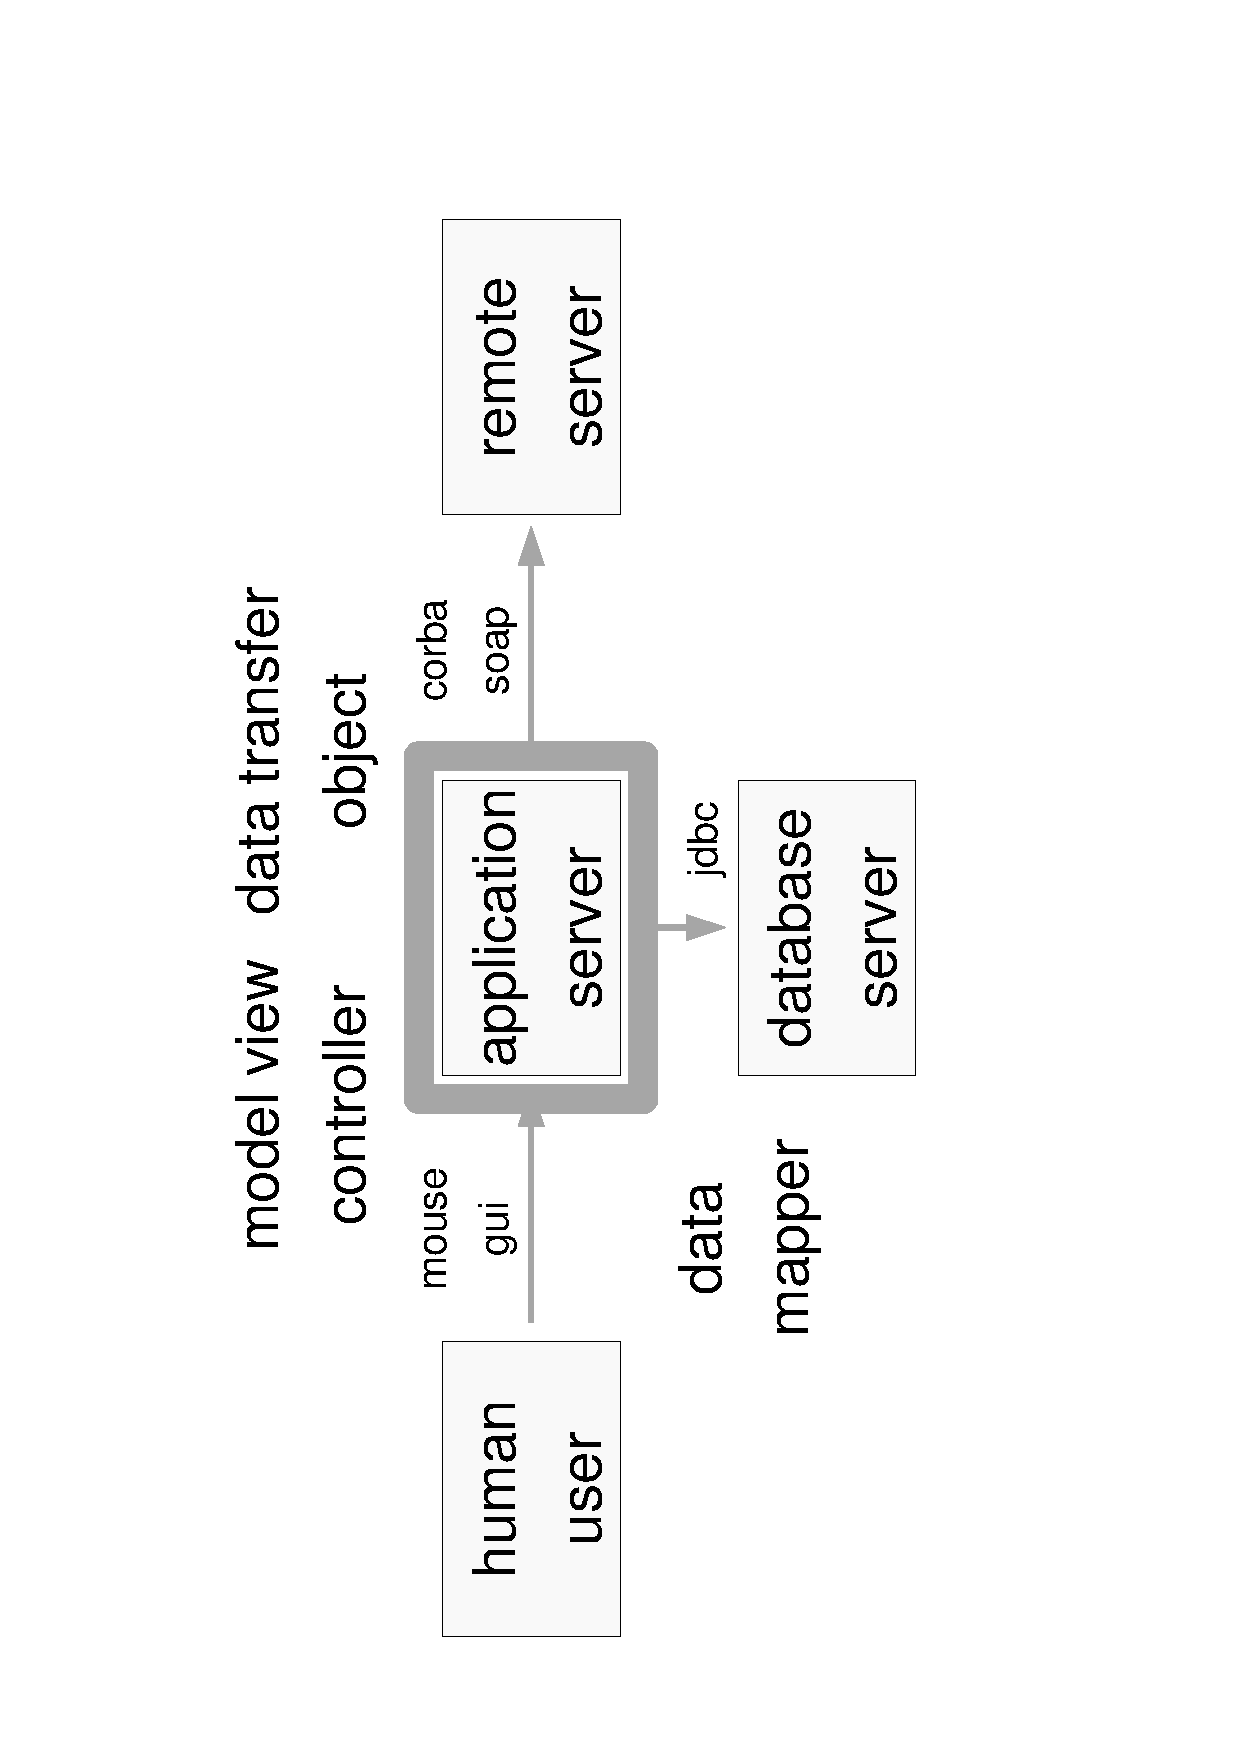
\includegraphics[scale=0.3,angle=-90]{graphic/communication.pdf}
        \caption{IT Environment with Server using Communication Patterns}
        \label{communication_figure}
    \end{center}
\end{figure}

Although software development has become a lot easier in the last decades, it is
still a big effort that should not be underestimated. One thing that application
developers have to care about much of their time is the \emph{Conversion}
between various kinds of (communication) models that a system has:

\begin{itemize}
    \item[-] Frontend (Communication with Human User)
    \item[-] Backend (Communication with Data Source)
    \item[-] Remote (Communication with Server)
    \item[-] Domain (Communication with own Knowledge)
\end{itemize}

The different mechanisms and patterns that have to be considered for such model
conversion often need to be implemented repeatedly, for each new application.
Some trials to unify all backend communication in a common \emph{Persistence Layer}
exist \cite{ambler}, but are remote- and frontend communication seldom considered
in a comparable way. Obviously, no current effort treats the frontend as just
another communication model that has to be \emph{sent} to the human user as
just another system.

The following sections will first reconsider three common communication
patterns, before embedding them into the classical model of logical system
layers (section \ref{layers_heading}). After that, a simplification is
suggested which finally leads to a new \emph{Translator Architecture} (first
introduced in \cite{hellerkunze}).

%
% $RCSfile$
%
% Copyright (c) 2002-2006. Christian Heller. All rights reserved.
%
% Permission is granted to copy, distribute and/or modify this document
% under the terms of the GNU Free Documentation License, Version 1.1 or
% any later version published by the Free Software Foundation; with no
% Invariant Sections, with no Front-Cover Texts and with no Back-Cover
% Texts. A copy of the license is included in the section entitled
% "GNU Free Documentation License".
%
% http://www.cybop.net
% - Cybernetics Oriented Programming -
%
% http://www.resmedicinae.org
% - Information in Medicine -
%
% Version: $Revision$ $Date$ $Author$
% Authors: Christian Heller <christian.heller@tuxtax.de>
%

\subsubsection{Pattern Simplification}
\label{pattern_simplification_heading}

The three communication patterns mentioned before had already been
reinvestigated for commonalities in \cite{hellerkunze}, which also embedded
them into the classical model of logical system layers (figure
\ref{simplification_figure}). For all kinds of communication, there is a:

\begin{itemize}
    \item[-] \emph{System} (Human User, Database, Remote Server)
    \item[-] \emph{Model} (View, ERM, DTO)
    \item[-] \emph{Translator} (Controller/ View Assembler, Data Mapper, DTO Assembler)
\end{itemize}

\begin{figure}[ht]
    \begin{center}
        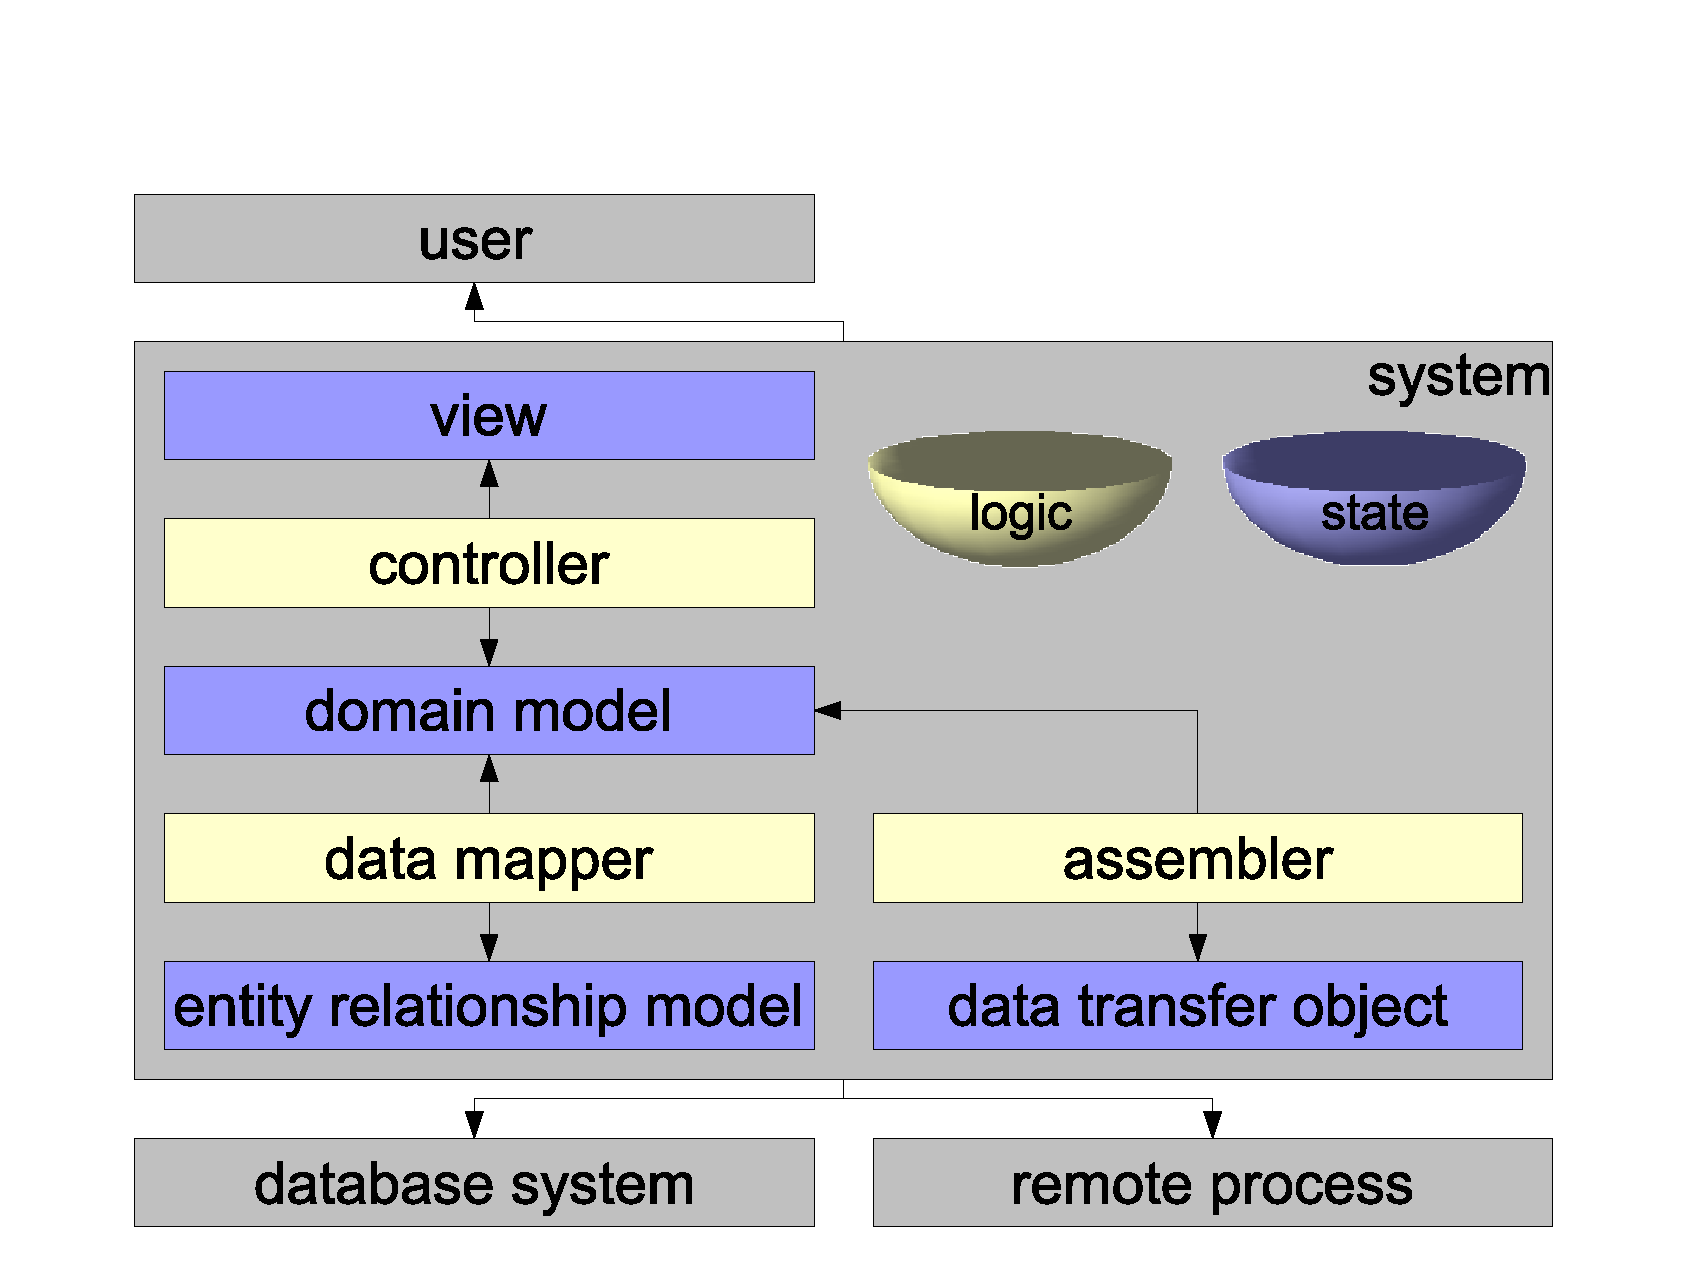
\includegraphics[scale=0.2]{vector/simplification.eps}
        \caption{Simplified Patterns in Layers}
        \label{simplification_figure}
    \end{center}
\end{figure}

All models represent certain states; all translators contain logic for
converting one state into another; all systems host their own, specific pool of
state- and logic knowledge. Realising this, a much clearer view on software
architectures can be retrieved.

Because domain models differ between systems, each system needs its own
translator models. Only communication models need to be agreed upon between
systems; they need to be understood by both communication partners.

%
% $RCSfile: communication_model.tex,v $
%
% Copyright (C) 2002-2008. Christian Heller.
%
% Permission is granted to copy, distribute and/or modify this document
% under the terms of the GNU Free Documentation License, Version 1.1 or
% any later version published by the Free Software Foundation; with no
% Invariant Sections, with no Front-Cover Texts and with no Back-Cover
% Texts. A copy of the license is included in the section entitled
% "GNU Free Documentation License".
%
% http://www.cybop.net
% - Cybernetics Oriented Programming -
%
% http://www.resmedicinae.org
% - Information in Medicine -
%
% Version: $Revision: 1.1 $ $Date: 2008-08-19 20:41:05 $ $Author: christian $
% Authors: Christian Heller <christian.heller@tuxtax.de>
%

\subsection{Communication Model}
\label{communication_model_heading}
\index{Communication Model}
\index{Medium of Communication}
\index{Domain Model}
\index{Transfer Model}
\index{Model Translator}
\index{Mapping Rules}
\index{Notation}
\index{Rules of Translation}
\index{Textual User Interface}
\index{TUI}
\index{Graphical User Interface}
\index{GUI}
\index{Web User Interface}
\index{WUI}
\index{x Datentr\"ager}
\index{xDT}
\index{Healthcare Xchange Protocol}
\index{HXP}
\index{Clinical Document Architecture}
\index{CDA}

As section \ref{communication_heading} pointed out, systems (alive or not)
never communicate directly, but always across the detour of an external
(transient or persistent) \emph{Medium}. This makes it necessary to use special
\emph{Communication Models}, since nearly always, only \emph{parts} of a
complete \emph{Domain Model} want to be exchanged. The use of communication
(transfer) models again, entails the use of model \emph{Translators}. Sowa
\cite{sowa} writes in his book \emph{Knowledge Representation}:

\begin{quote}
    In computer science, there is no end to the number of specialized notations.
    Besides the hundreds of programming languages, there are diagrams for circuits,
    flowcharts, parse trees, game trees, Petri nets, PERT charts, neural networks,
    design languages, and novel notations that are invented whenever two
    programmers work out ideas at the blackboard. Musical notation \ldots\
    is an example of a complex language that is both precise and human factored.
    As long as the mapping rules are defined, all of these notations can be
    automatically translated to or from logic.
\end{quote}

\begin{figure}[ht]
    \begin{center}
        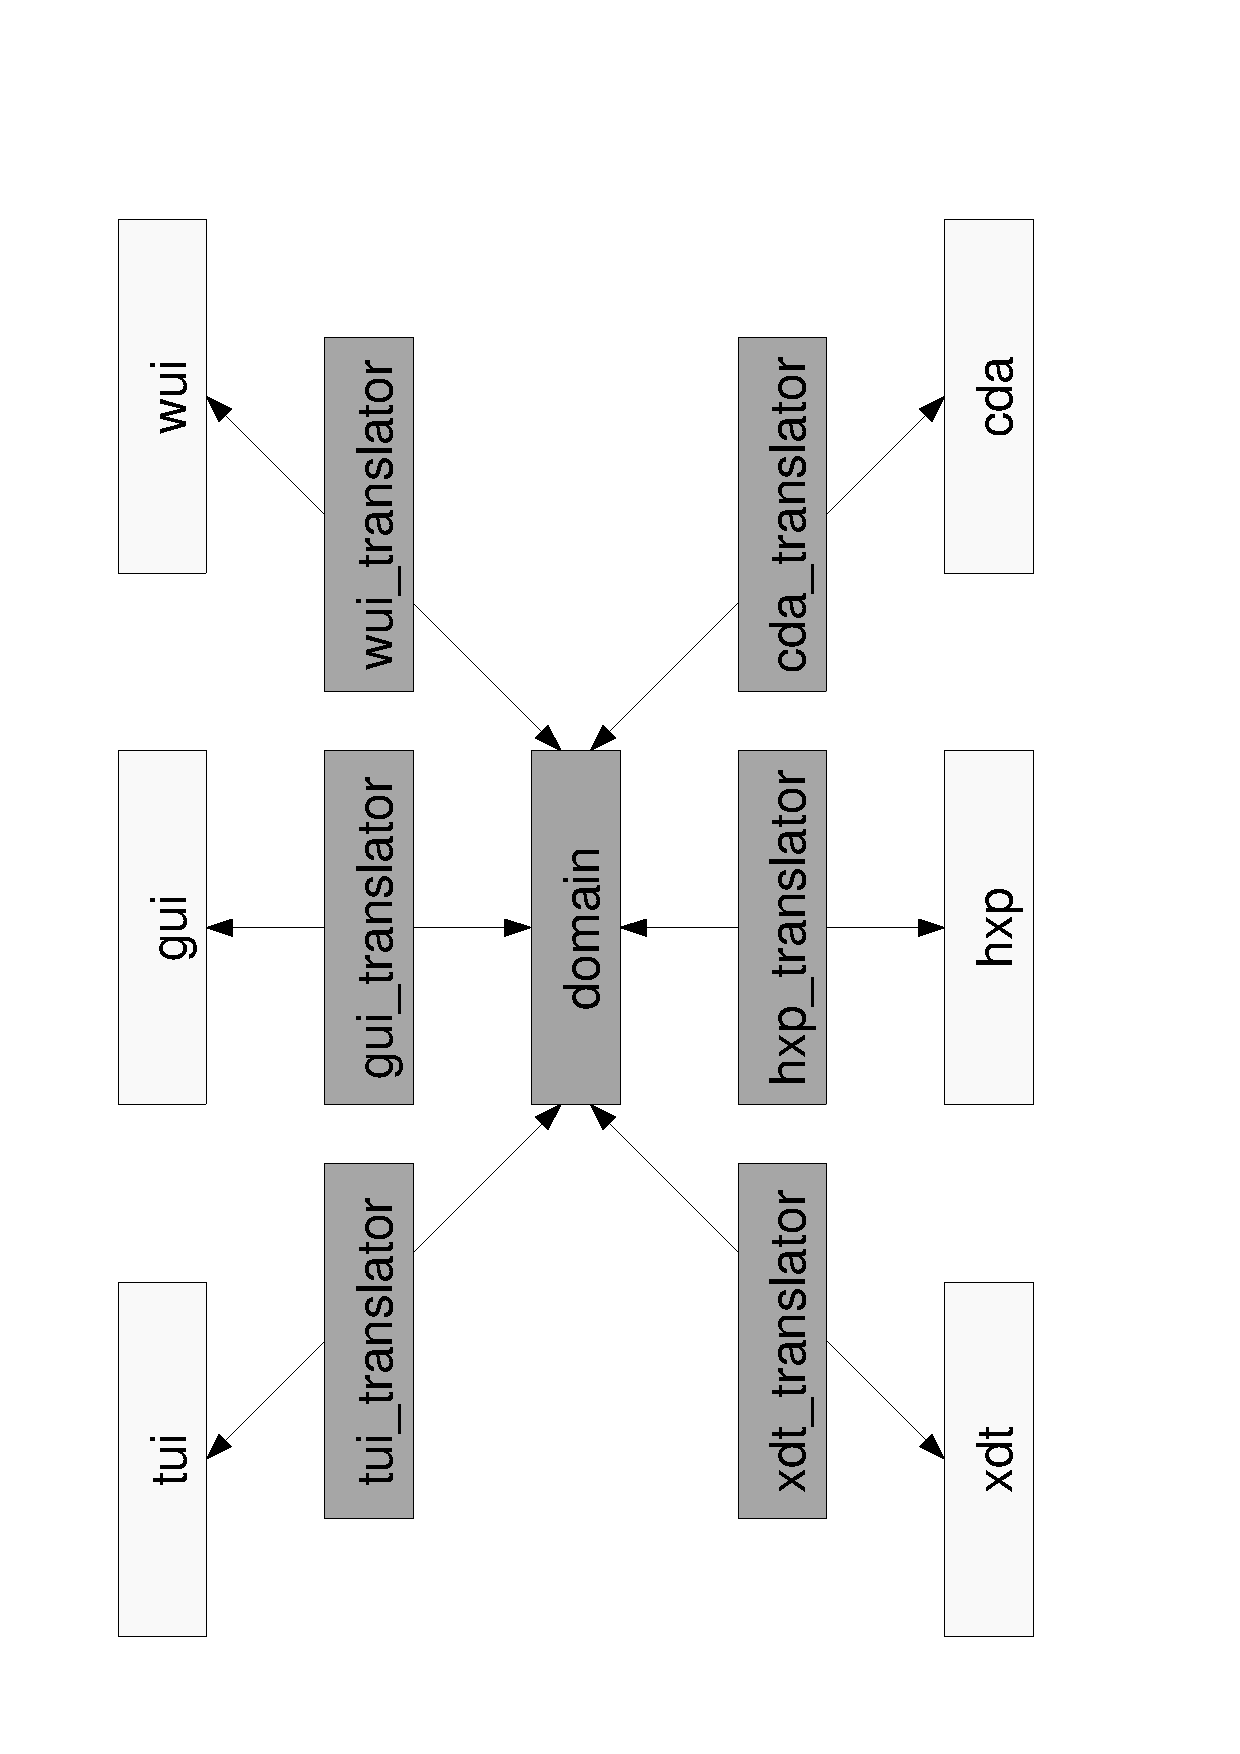
\includegraphics[scale=0.3,angle=-90]{graphic/translators.pdf}
        \caption{Different Kinds of Model Translators}
        \label{translators_figure}
    \end{center}
\end{figure}

Although he does not talk of \emph{Domain-} and \emph{Communication Models},
but of \emph{Notations}, Sowa obviously means the same: Any kind of abstract
model can be translated into any other kind, as long as the translation
\emph{Rules} are defined. Model \emph{Translators} are able to map domain model
data to transfer model data. Depending on which communication style is used,
different translators with different rules need to be applied.

Figure \ref{translators_figure} shows a number of possible model translators,
for a: \emph{Textual User Interface} (TUI), \emph{Graphical User Interface}
(GUI) and \emph{Web User Interface} (WUI) as well as for the German standard
file format for exchanging medical data called \emph{x Datentr\"ager} (xDT),
the \emph{Healthcare Xchange Protocol} (HXP) and HL7's exchange format called
\emph{Clinical Document Architecture} (CDA). More on these standards in chapter
\ref{res_medicinae_heading}.

Many application systems have exactly one domain model but transfer models of
arbitrary type should be addable anytime. Translators only know how to
translate between the domain model and a special transfer model, of course in
both directions. \emph{Direct} translation between transfer models is an
exception; it is possible but better done \emph{via} the domain model.

The type of transfer model is independent from the communication mechanism
used. The usage of a \emph{Graphical User Interface} (GUI) model, for example,
is not necessarily limited to human-computer interaction. It could very well be
used for data transfer between remote computers, as long as both systems know
how to translate that model.

%
% $RCSfile$
%
% Copyright (c) 2002-2006. Christian Heller. All rights reserved.
%
% Permission is granted to copy, distribute and/or modify this document
% under the terms of the GNU Free Documentation License, Version 1.1 or
% any later version published by the Free Software Foundation; with no
% Invariant Sections, with no Front-Cover Texts and with no Back-Cover
% Texts. A copy of the license is included in the section entitled
% "GNU Free Documentation License".
%
% http://www.cybop.net
% - Cybernetics Oriented Programming -
%
% http://www.resmedicinae.org
% - Information in Medicine -
%
% Version: $Revision$ $Date$ $Author$
% Authors: Christian Heller <christian.heller@tuxtax.de>
%

\subsubsection{Logic manipulates State}
\label{logic_manipulates_state_heading}

According to the observations made in the work described in this article, there
are two kinds of knowledge: \emph{States} and \emph{Logic}. While the former
may be placed in a spatial dimension, the latter is processed as sequence over
time. Often, logic is labelled \emph{dynamic} behaviour -- but only the
\emph{execution} of a rule of logic is dynamic, \emph{not} the rule itself
(\emph{static}).

Rules of logic translate input- into output states. What characterises a system
is how it applies logic knowledge to translate state knowledge \cite{heller2002}.
Yet how to imagine a knowledge model consisting of state- as well as logic
parts? Following an example. The famous \emph{Model View Controller} (MVC)
pattern was extended by the \emph{Hierarchical MVC} (HMVC) pattern towards a
hierarchy of \emph{MVC Triads} \cite{cai}. The omnipresence of hierarchies in
the MVC was demonstrated in \cite{hellerbohl}.

\begin{figure}[ht]
    \begin{center}
        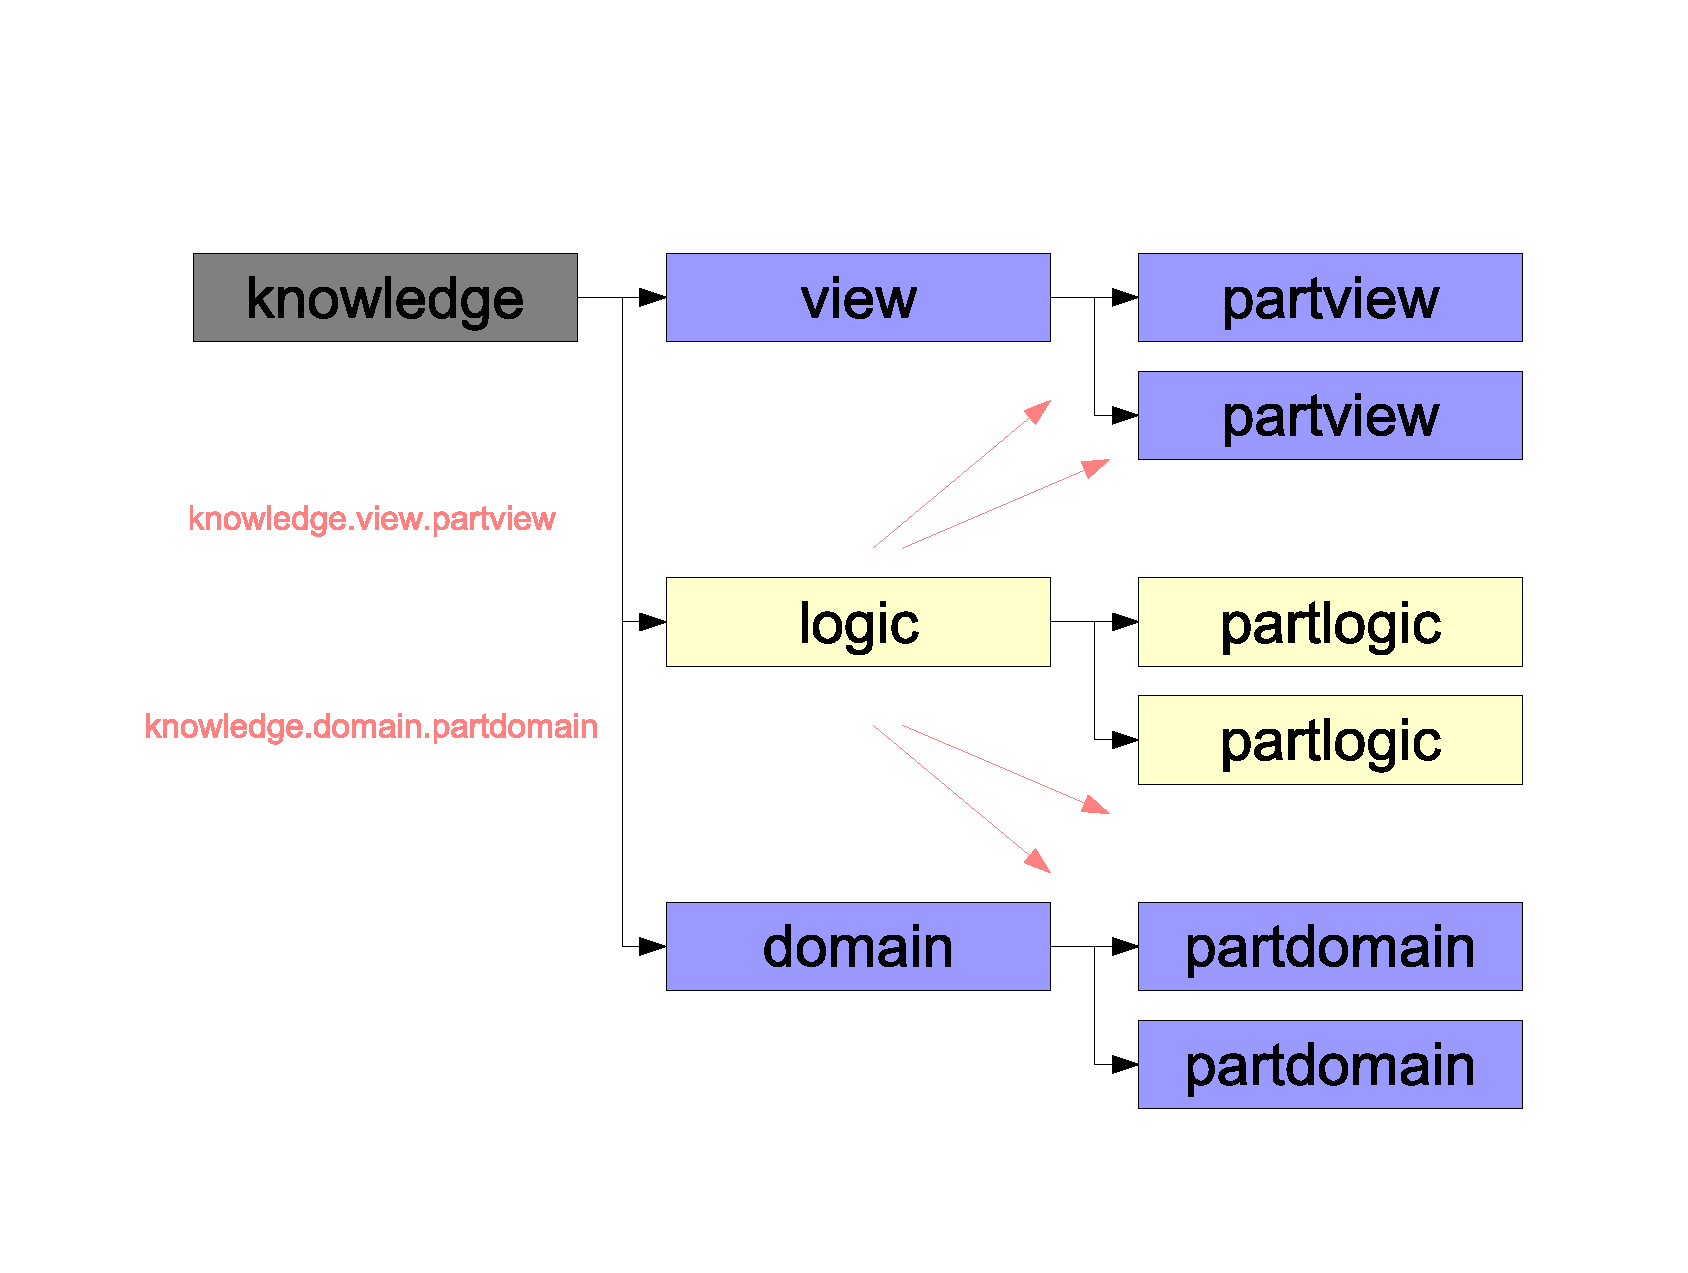
\includegraphics[scale=0.2]{vector/mvctree.eps}
        \caption{Logic manipulating States}
        \label{mvctree_figure}
    \end{center}
\end{figure}

Figure \ref{mvctree_figure} shows the three parts: \emph{Domain} (Model),
\emph{View} and \emph{Logic} (Controller) of an (adapted) MVC pattern as
independent branches of one common knowledge tree, as existent at system
runtime in memory. Each of them represents a concept on its own. The logic
model, however, is allowed to access and change the view- and domain model; it
is able to link different knowledge models. But view- and domain model,
representing states, are not allowed to manipulate logic. In other words: The
dependencies between logic- and state models are \emph{unidirectional}.

An innovation is that logic knowledge gets manipulatable. A logic model
(algorithm) cannot only access and change state-, but also logic models, even
itself! Because models modified in that manner can be made persistent in form
of CYBOL knowledge templates (section \ref{cybol_heading}), and be reloaded the
next time an application starts, this may be seen as a kind of
\emph{Meta Programming}, which \cite{wikipedia} defines as: \textit{the writing
of programs that write or manipulate other programs (or themselves) as their
data.}

The clear separation of states and logic into discrete models avoids unwanted
dependencies as caused by the bundling of attributes and methods in OOP. All
that would be needed to make a CYBOP system work with new state models, is the
corresponding translation logic. Translators \cite{hellerkunze} simplify
architectures and unify communication.

